% !TEX root = main.tex

\section{Yields determination}
\label{sec:massFits}

An extended unbinned maximum likelihood fit to the reconstructed $B_s$ mass of the selected events is performed in order to determine the signal and background yields.
The invariant mass $m(D_s h \pi \pi)$ is determined from a DTF constraining the mass of the $D_s$ to the PDG value and the position of the PV. 
The probability density functions (PDFs) used to describe the signal and background components are described in the following.

Due to different mass resolutions, we perform the invariant mass fits simultaneously for each data-taking period and each trigger category. 
We further introduce four $D_s$ final state categories:
$D_s \to \phi \pi$, $D_s \to K^*(892) \pi$, $D_s \to \pi \pi \pi$ and $D_s \to K h \pi$
to account for different signal purities. 
The $D_s \to K h \pi$ category combines the two $D_s$ decay channels with the lowest statistics: $D_s \to K K \pi$ (non-resonant) and $D_s \to K \pi \pi$.
This amounts to 16 categories in total.



\subsection{Signal model}
\label{subsec:signalModel}

The signal $B_s$-mass distribution of both $\Bs\to\Ds\kaon\pion\pion$ and $\Bs\to\Ds\pion\pion\pion$  is modeled using a Johnson's SU function \cite{10.2307/2332539}, which 
results from a variable transformation of a normal distribution to allow for asymmetric tails:
\begin{align}
\mathcal J(x\vert\mu,\sigma,\nu,\tau) &=
\frac{e^{- \frac{1}{2} r^2}}{2\pi \cdot c \cdot \sigma \cdot \tau \cdot \sqrt{z^2+1}} \\
% \frac{\delta}{\sigma 2\pi \sqrt{1+(\frac{m_{\Bs}-\mu}{\sigma})^{2}}} exp \left(-\frac{1}{2}[\gamma + \delta Argsh (\frac{m_{\Bs} - \mu}{\sigma})^{2}]\right).
r &= - \nu + \frac{\text{asinh}(z)}{\tau} \\
z & = \frac{x-(\mu - c \cdot \sigma \cdot e^\tau \text{sinh}(\nu\cdot \tau))}{c \cdot \tau} \\
c &= \frac{e^{\tau^2}-1}{2\sqrt{e^{\tau^2} \cdot \text{cosh}(2 \nu \cdot \tau)+1}} .
\label{eq:RooJohnsonSU}
\end{align}
It is conveniently expressed in terms of the central moments up to order four: 
The mean of the distribution $\mu$, the standard deviation $\sigma$,
the skewness $\nu$ and the kurtosis $\tau$.
%The sign of $\gamma$ in Eq. \ref{eq:RooJohnsonSU} determines whether the tail is located at lower ($\gamma > 0$) or higher ($\gamma < 0$) invariant mass values than the mean $\mu$ of the gaussian function 
%and $\delta$ describes the (a)symmetry of the fitted distribution. Higher values of $\delta$ result in a more symmetric, gaussian-like function.  
%Another Johnson SU function function is used to account for the contribution of the $\B^{0}\to\Ds\kaon\pion\pion$ decay, which is also present in the $m(\Ds\kaon\pion\pion)$ spectrum.
The tail parameters $\nu$ and $\tau$ are fixed to the values obtained by a fit to the invariant mass distribution of simulated events shown in Fig~\ref{fig: BsMassShapes}. 
\begin{figure}[b]
\centering
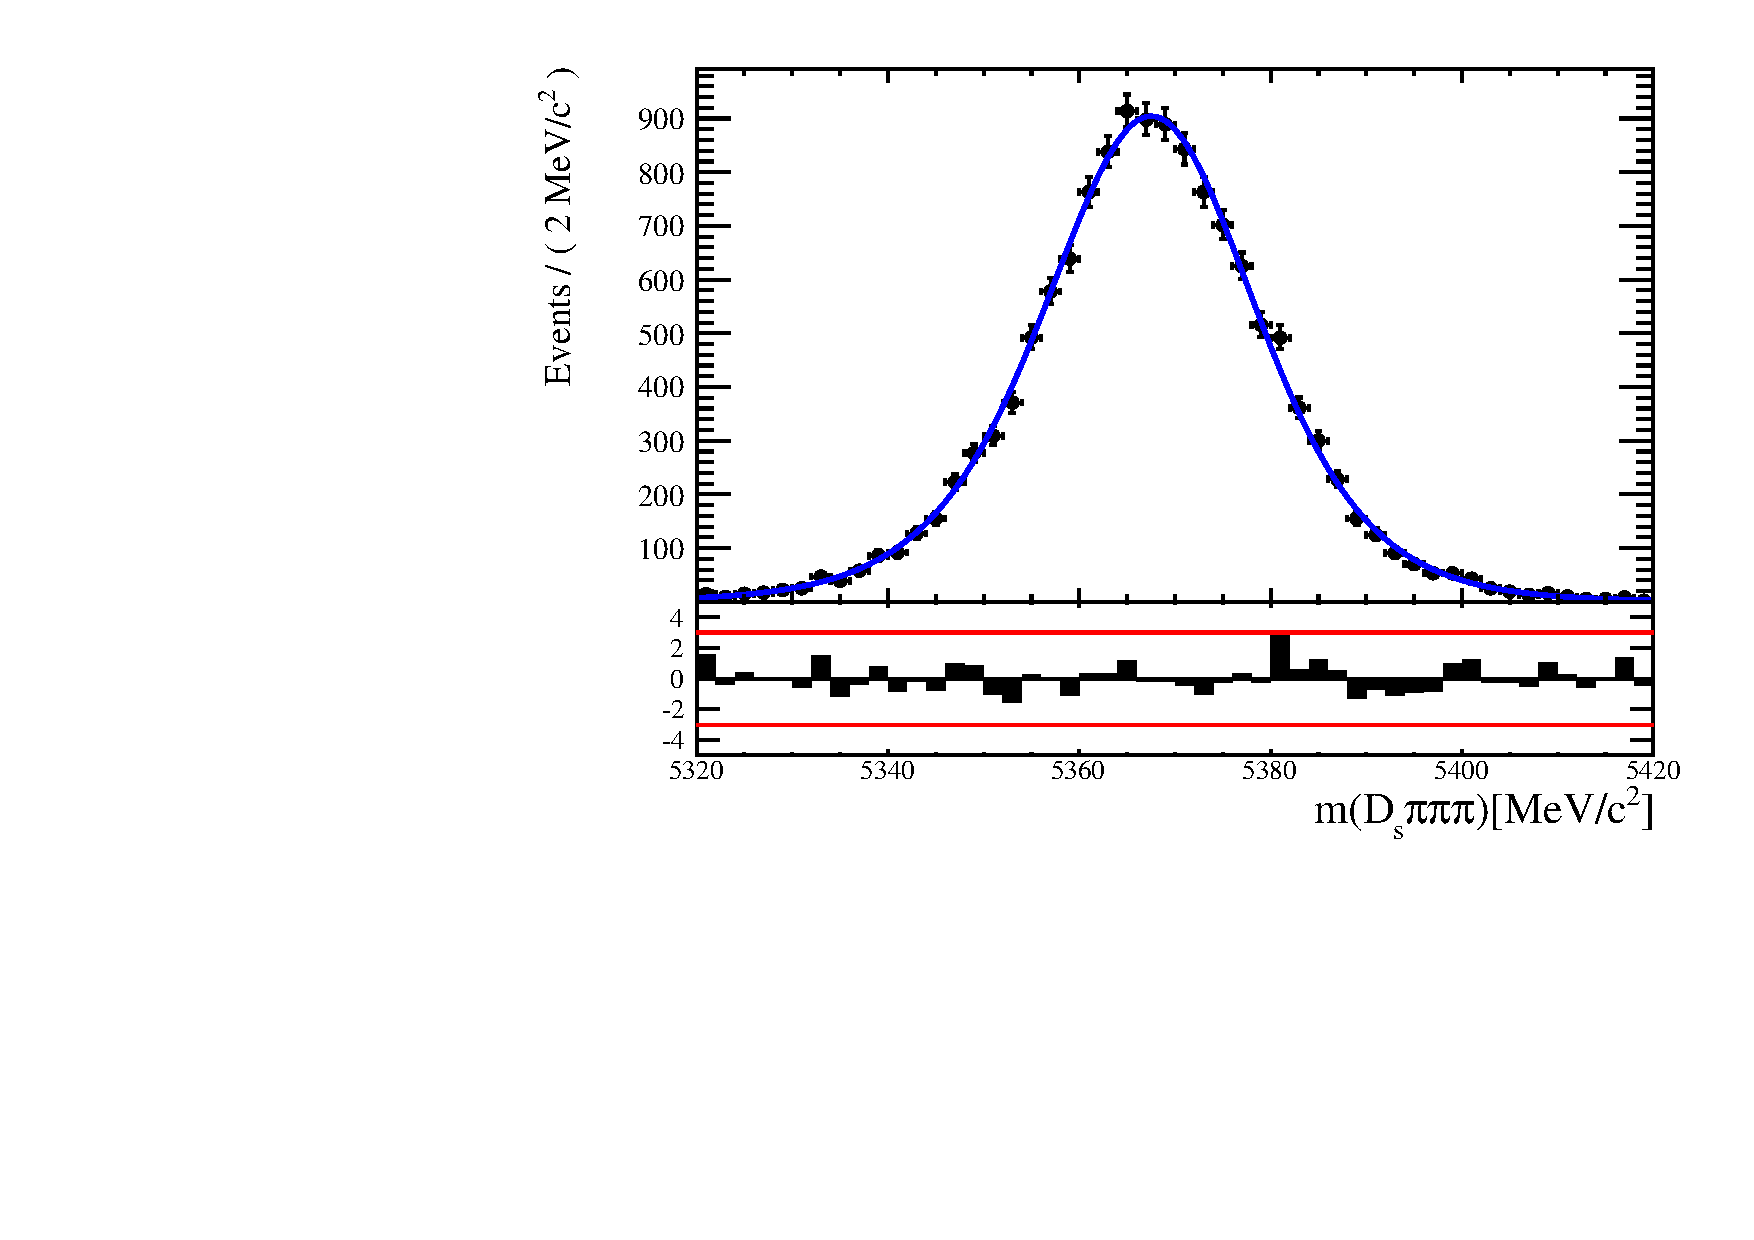
\includegraphics[height=!,width=0.32\textwidth]{figs/MassFit/normMC_pull.pdf} 
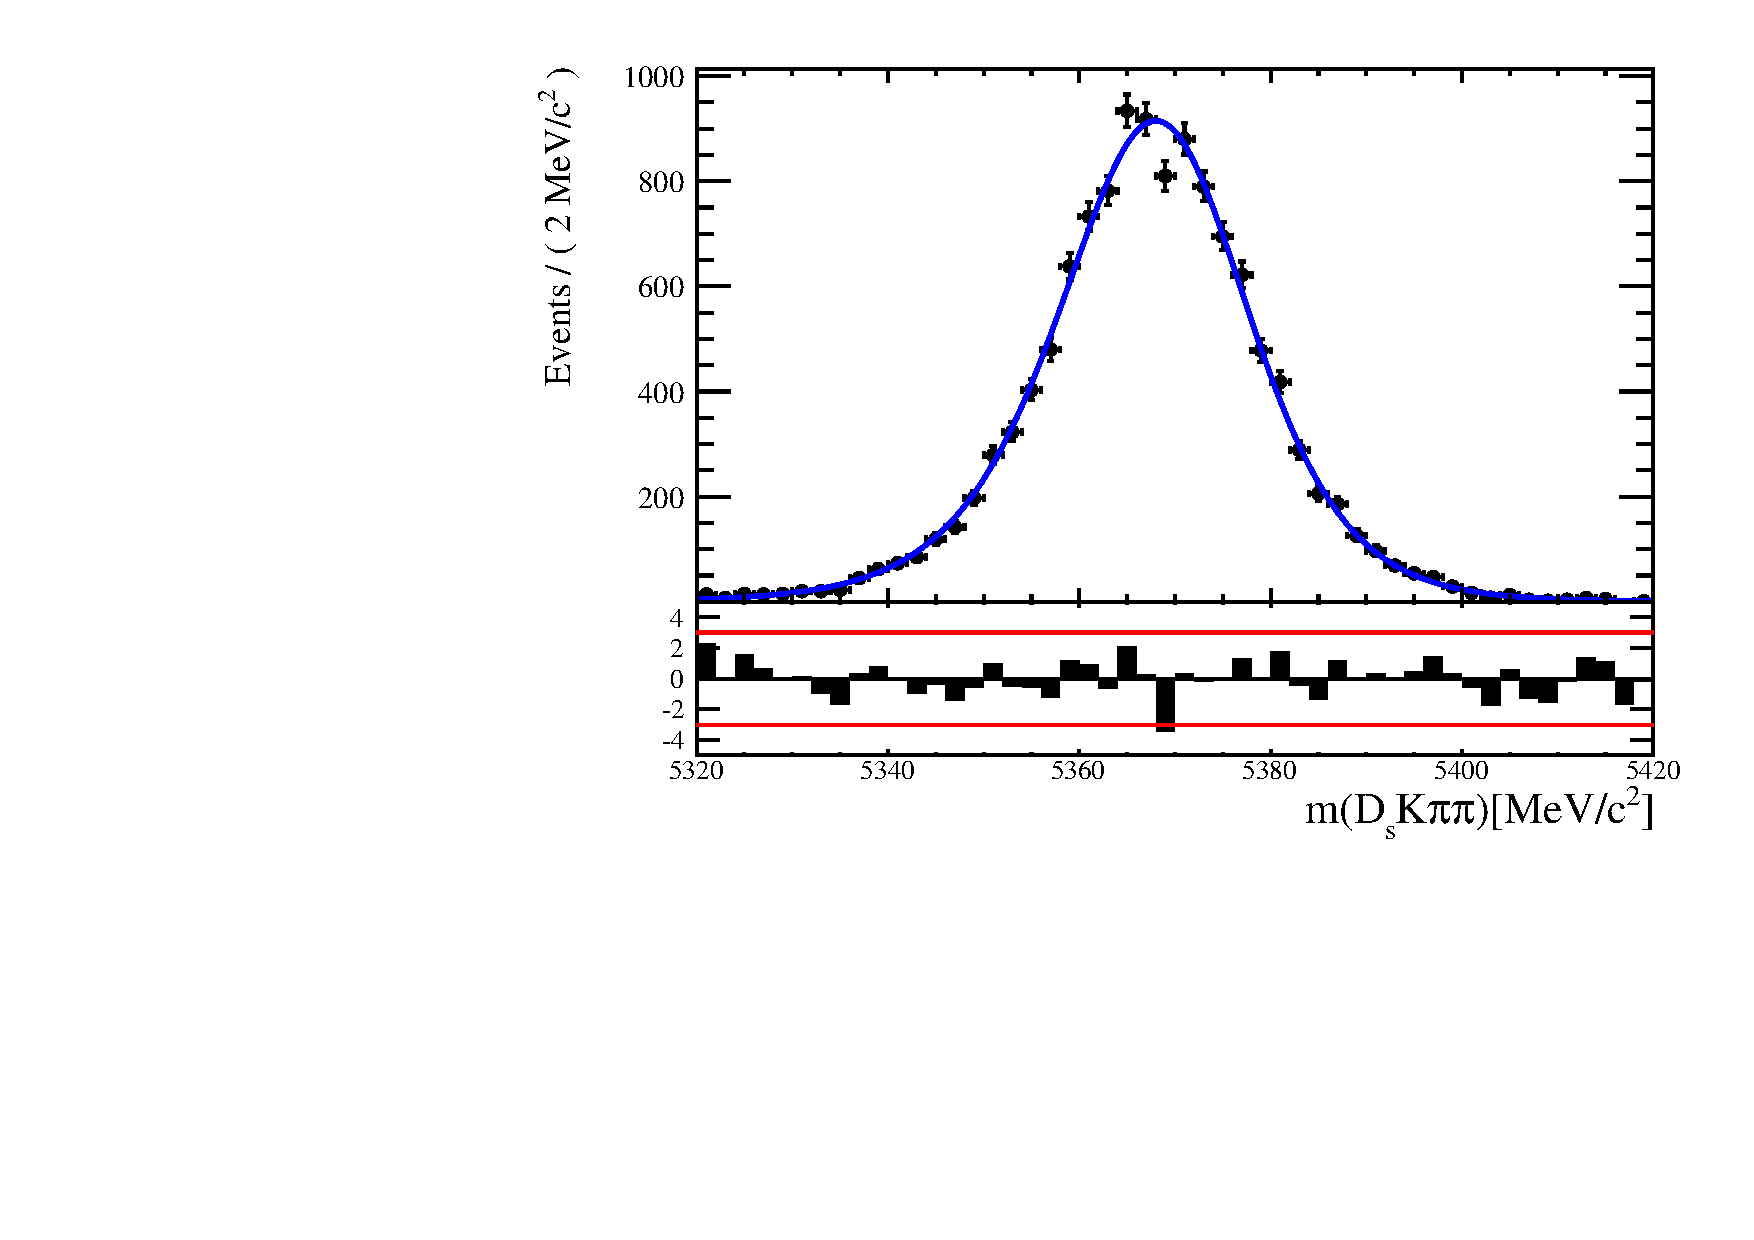
\includegraphics[height=!,width=0.32\textwidth]{figs/MassFit/signalMC_pull.pdf}
\caption{Invariant mass distributions of simulated (left) $\Bs\to\Ds\pion\pion\pion$ and (right) $\Bs\to\Ds\kaon\pion\pion$ events. A fit with a Johnson's SU PDF is overlaid.}
\label{fig: BsMassShapes}
\end{figure}
To account for differences between simulation and real data, linear scaling factors for the mean $\mu$ and width $\sigma$ are determined in the fit to $\Bs\to\Ds\pion\pion\pion$ data  
and later fixed in the fit to $\Bs\to\Ds\kaon\pion\pion$ decays. 
The scale factors are determined separately for each data-taking period and each trigger category.


\subsection{Background models} 
\label{subsec:bkgModel}

After the full selection the following residual background components have to be accounted for: \\

\noindent \textbf{Combinatorial background}  \\
The combinatorial background is described by a second order polynomial,
whose parameters are determined, for each $D_s$ final state separately, in the fit to data.
For systematic studies an exponential PDF is used.
\\

\noindent\textbf{Peaking $B_d$ background}  \\
Decays of $B_d$ mesons into the $D_s h \pi \pi$ final state are described by the $B_s$ signal PDF where the mean is shifted by the known mass difference $m_{B_s} - m_{B_d}$\cite{PDG2016}.
\\

\noindent \textbf{Partially reconstructed background}  \\
Partially reconstructed $\Bs\to D_s^{*}\pi\pion\pion$ decays, with $D_s^{*}\to\Ds\gamma$ or $D_s^{*}\to\Ds\piz$,
are expected to be peaking lower than signal in the $m(\Ds\pion\pion\pion)$ spectrum with large tails due to the %missing 
momentum carried away by the not reconstructed $\piz$ or $\gamma$. 
An empirical description for the shape of this contribution is derived from a $\Bs\to D_s^{*}\pi\pion\pion$ MC sample subject to the nominal $\Bs\to D_s\pi\pion\pion$ selection.
Figure \ref{fig:bgkShapes} (top) shows the respective reconstructed $m(D_s\pi\pi\pi)$ distribution.
A sum of three bifurcated Gaussian functions (\ie Gaussian functions with different widths on the left and the right side of the maximum value) is used to describe it.
In the fit to data, all parameters are fixed to the ones obtained from MC except for the parameter which describes the width of the right tail of the distribution to account for
data-simulation differences in mass resolution.
The equivalent $\Bs\to D_s^{*}K\pion\pion$ component contributing to the $\Bs\to D_s K\pion\pion$ data sample is described by the same PDF with the right tail fixed to the 
$\Bs\to D_s \pi\pion\pion$ result.

Contributions from $\Bz\to D_s^{*}K\pion\pion$ decays are modeled with the $\Bs\to D_s^{*}K\pion\pion$ PDF  shifted by $m_{\Bs} - m_{\Bz}$. \\
%Contributions from $\Bz\to D_s^{*}h\pion\pion$ decays where initially considered as well (modeled with the same PDF as $\Bs\to D_s^{*}h\pion\pion$ decays shifted by $m_{\Bs} - m_{\Bz}$) but were found to be negligible within the considered mass range. \\
%The yields of both contributions are directly determined in the nominal fit. \\

\noindent\textbf{Misidentified background}  \\
A small fraction of $B_s \to D_s^- \pi^+ \pi^+ \pi^-$ and $\Bs\to D_s^{*}\pi^+ \pi^+ \pi^-$ decays, where one of the pions is misidentified as a kaon, contaminate the 
$\Bs\to D_s K^+ \pi^+ \pi^-$ sample.
To determine the corresponding background shapes, we use simulated events passing the nominal selection
except for the PID cuts on the bachelor $\pi^+$ tracks. 
The \textsf{PIDCalib} package is used to determine the $p_T,\eta$-dependent $\pi^+\rightarrow K^+$ misidentification probability for each pion. 
%For every candidate in our MC sample, a (momentum) $\ptot$ and (pseudorapidity) $\eta$-dependent event weight is computed and assigned. 
We change the particle hypothesis from pion to kaon for the pion with the higher misidentification probability and recompute the invariant $\Bs$ mass, $m(D_s^- \pi^+_K \pi^+ \pi^- )$. 
Similarly, the invariant masses $m(\pi^+_K \pi^+ \pi^- )$ and $m(\pi^+_K \pi^-)$ are recomputed and required to be within the considered phasespace region.
The background distributions are shown in Fig.~\ref{fig:bgkShapes} (middle, bottom) and modeled by the sum of three Crystal Ball functions. 
\newpage
The expected yield of misidentified $\Bs\to\Ds\pion\pion\pion$ ($\Bs\to D_s^{*}\pi^+ \pi^+ \pi^-$) candidates in the $\Bs\to\Ds K\pion\pion$ sample is computed 
by multiplying the fake rate (within the considered $B_s$ mass range) of $0.63 \pm 0.01\%$ ($0.55 \pm 0.02\%$) 
for Run-I 
and $0.33 \pm 0.01\%$ ($0.24 \pm 0.01\%$) 
for Run-II
 %, which is derived from \textsf{PIDCalib}, 
by the $\Bs\to\Ds\pion\pion\pion$ ($\Bs\to D_s^{*}\pi^+ \pi^+ \pi^-$) yield as determined in the mass fit to the $\Bs\to\Ds\pion\pion\pion$ data sample.
The yields are corrected for the PID($\pip$)$<0$ requirement which has an efficiency of $77.1 \pm 0.1 \%$ for Run-I and $81.0 \pm 0.1 \%$ for Run-II data.  
The $\Bs\to D_s^{*}\pi^+ \pi^+ \pi^-$ yield is additionally corrected for the efficiency of the cut $m(\Ds K\pion\pion)>5200\mev$ evaluated on MC.
In the fit to data, the misidentified background yields are fixed to the predicted ones.
%In the same way as mentioned above, we can determine the rate of misidentified, partially reconstructed $\Bs\to\Ds^{*}\pion\pion\pion$ decays in our sample of $\Bs\to\Ds\kaon\pion\pion$ decays using \textsf{PIDCalib} and a MC sample of $\Bs\to\Ds^{*}\pion\pion\pion$ events. The invariant mass distribution we obtain when we exclude the $\gamma$/$\piz$, flip the the particle hypothesis $\pion\rightarrow\kaon$ and apply the event weights given by the fake rate, is shown in Fig.~\ref{fig:bgkShapes} (right). 
%The fit of two Crystal Ball functions to this distribution is overlaid. 
%The yield of this contribution is determined from the yield of $\Bs\to\Ds^{*}\pion\pion\pion$ candidates in the nominal mass fit of our normalization channel, multiplied by the misID probability of $\propto 3.6\%$.

We consider the $\Bs\to D_s K\pion\pion$ and $\Bs\to D_s^{*}K\pion\pion$ components contributing to the $\Bs\to D_s \pi\pion\pion$ data sample to be negligible 
due to the low branching fractions and the tight PID cuts on the bachelor pions.

\begin{figure}[b]
\centering
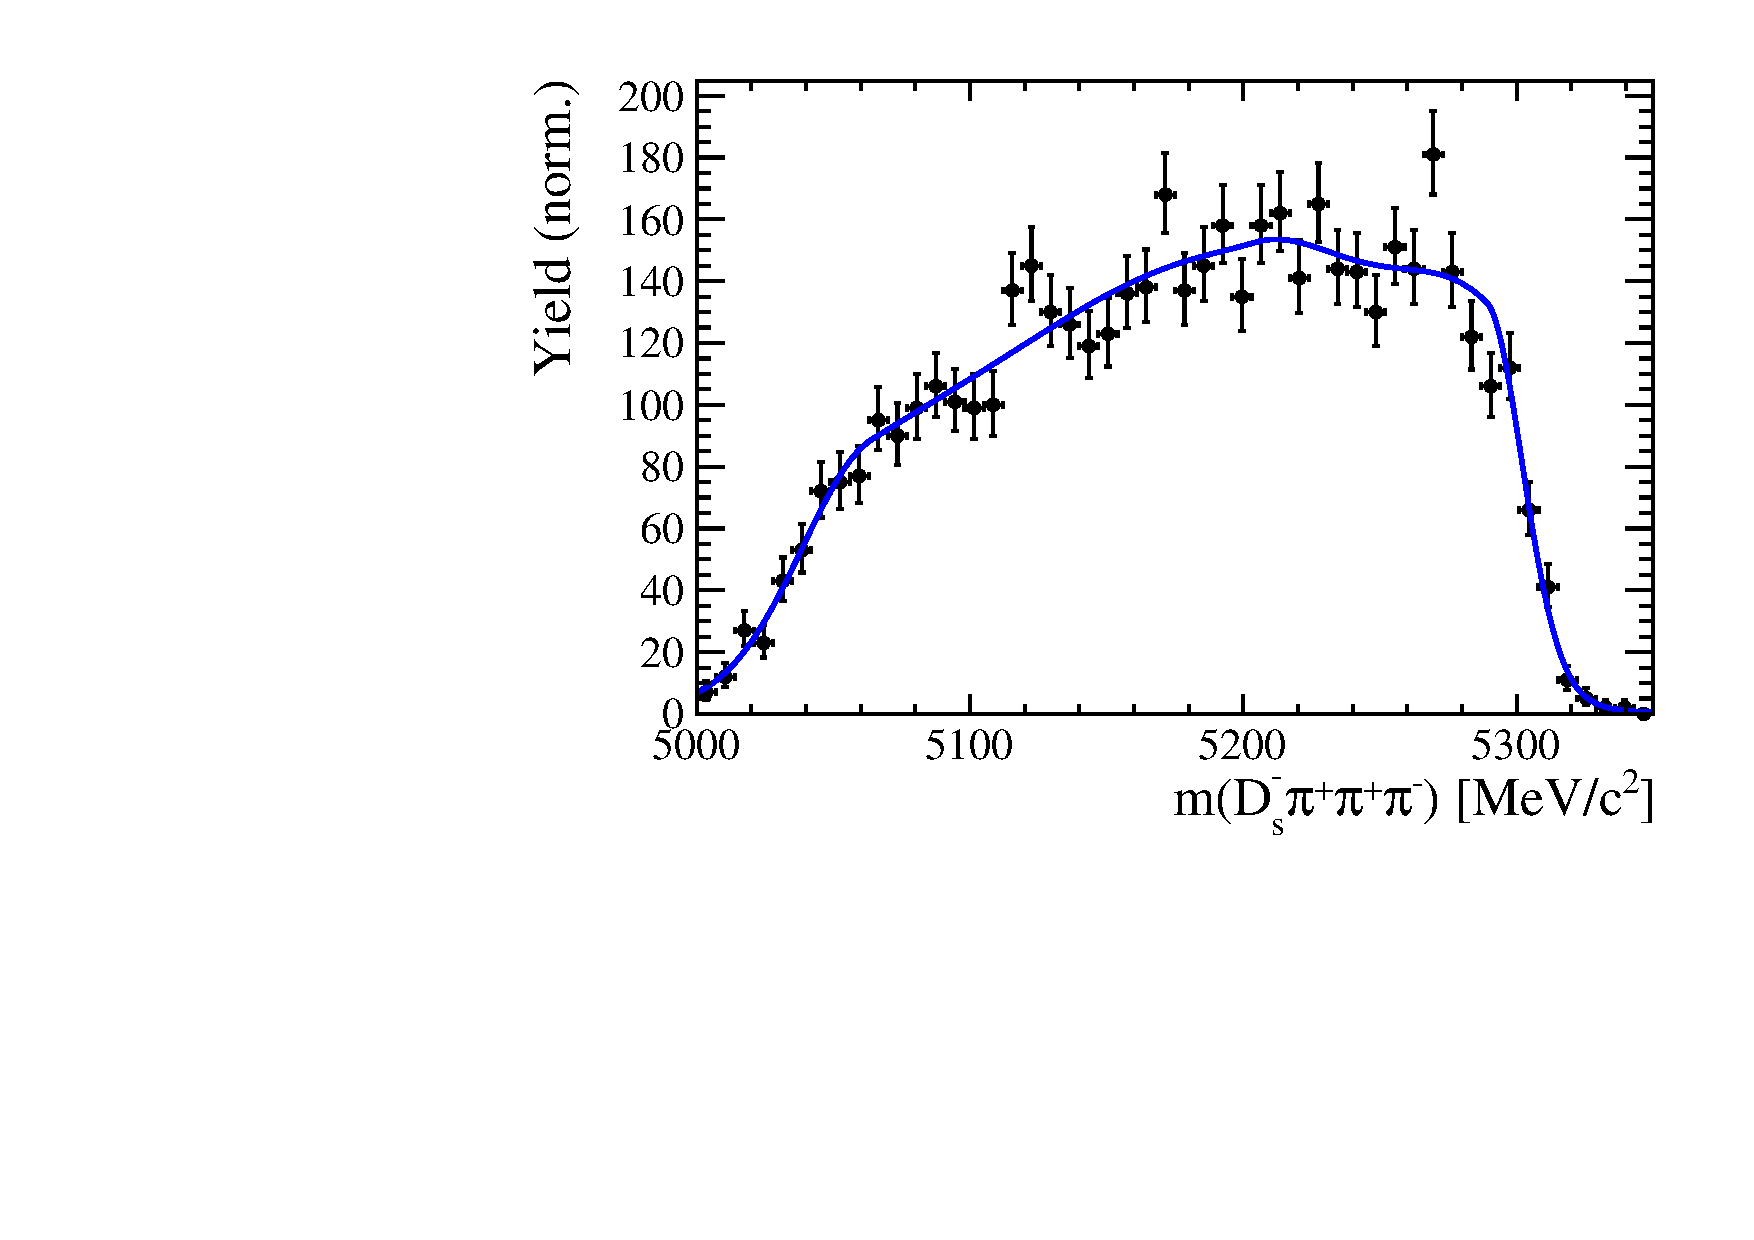
\includegraphics[height=!,width=0.4\textwidth]{figs/MassFit/BkgShape/Bs2Dsstartpipipi.pdf}

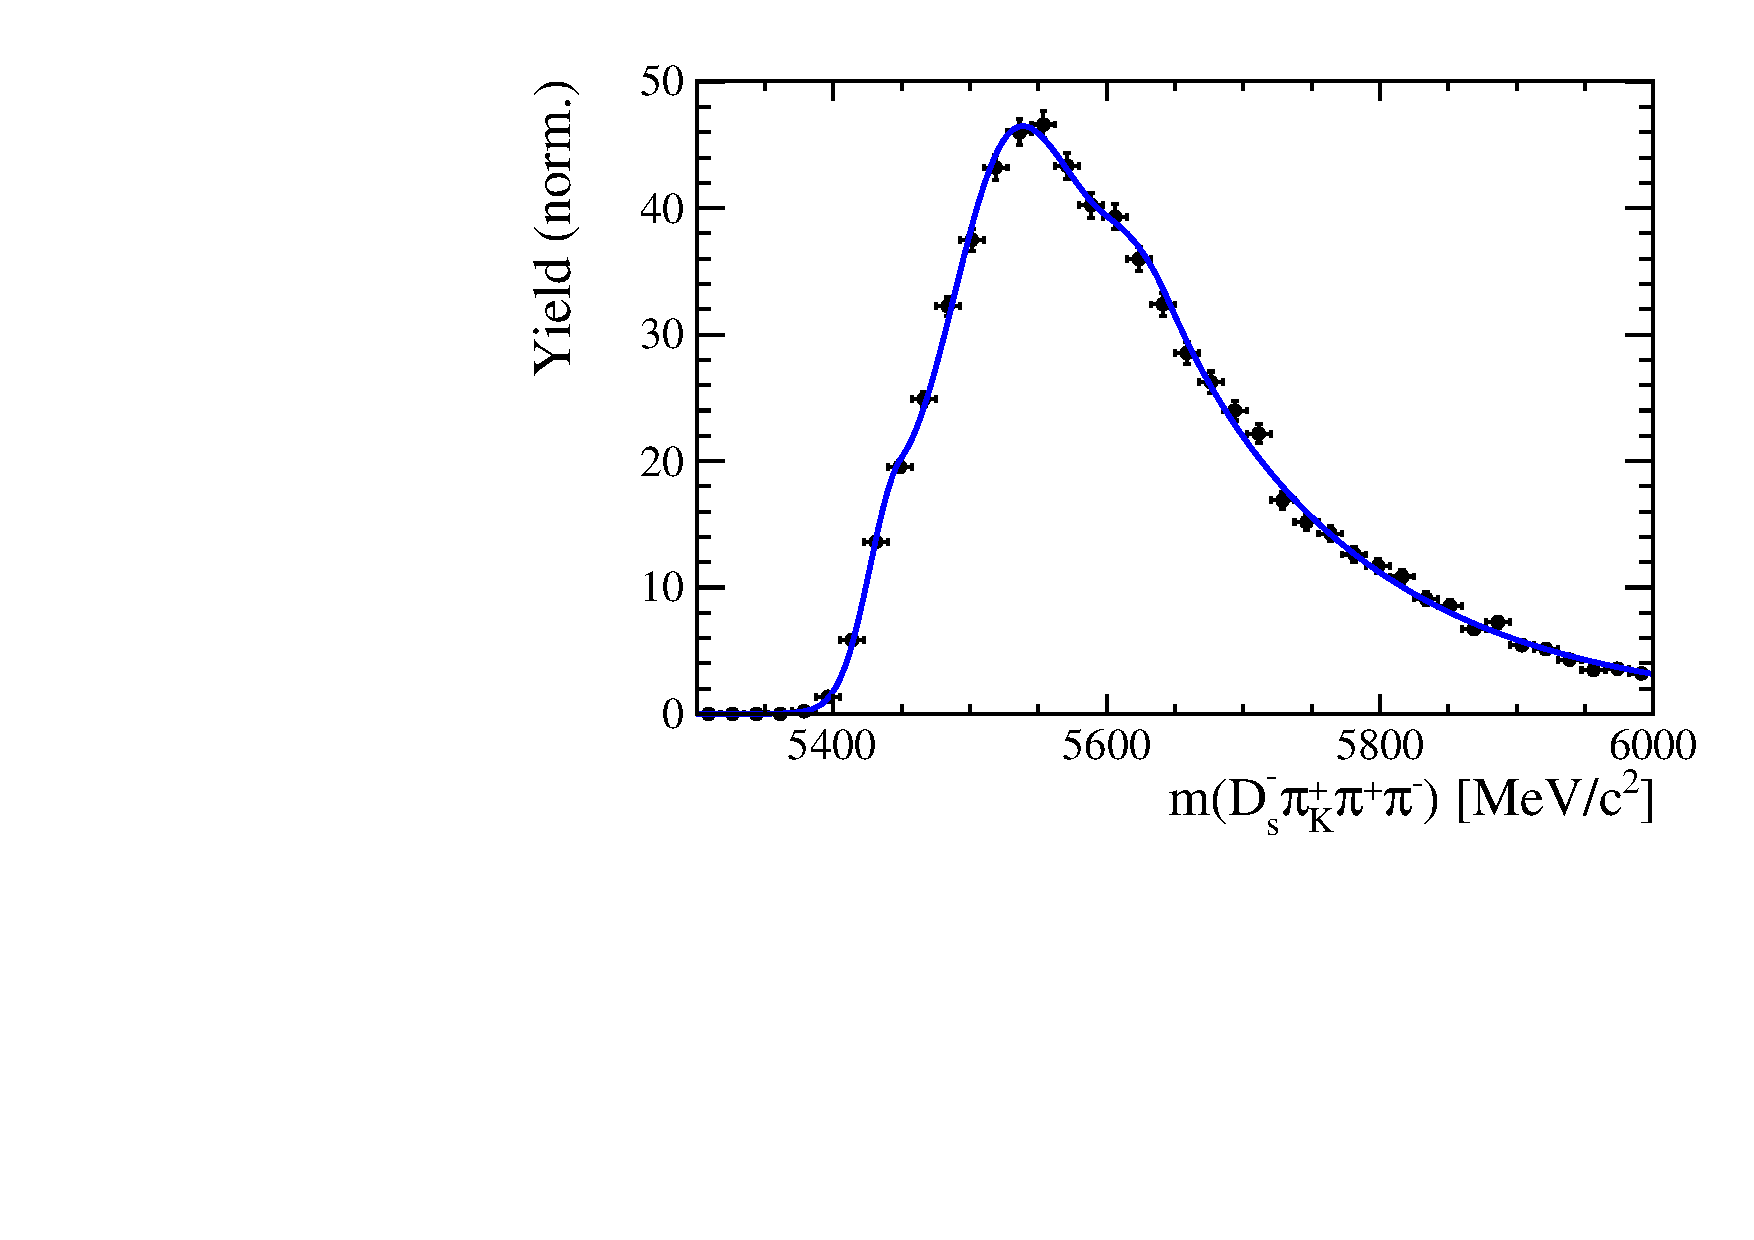
\includegraphics[height=!,width=0.4\textwidth]{figs/MassFit/BkgShape/Bs2Dspipipi_as_DsKpipi_Run1.pdf}
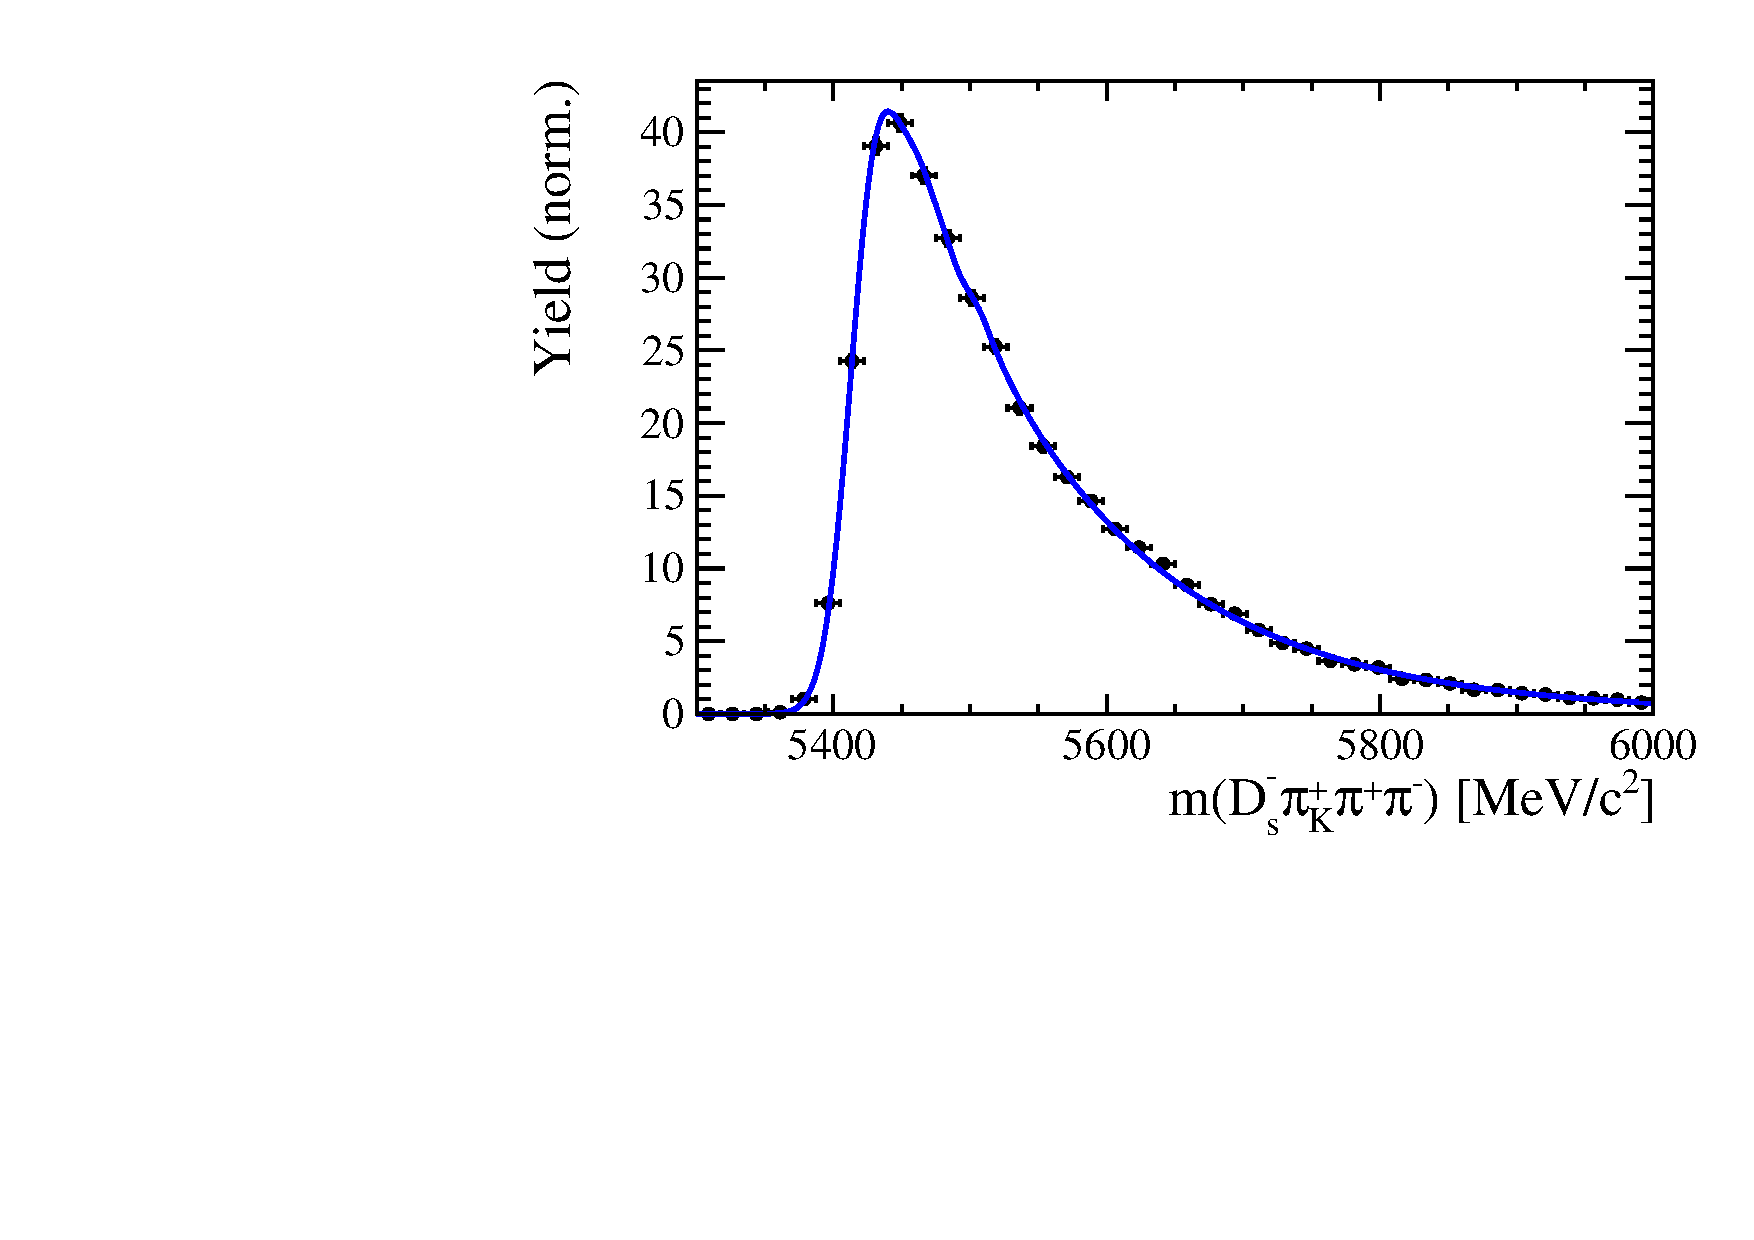
\includegraphics[height=!,width=0.4\textwidth]{figs/MassFit/BkgShape/Bs2Dspipipi_as_DsKpipi_Run2.pdf}

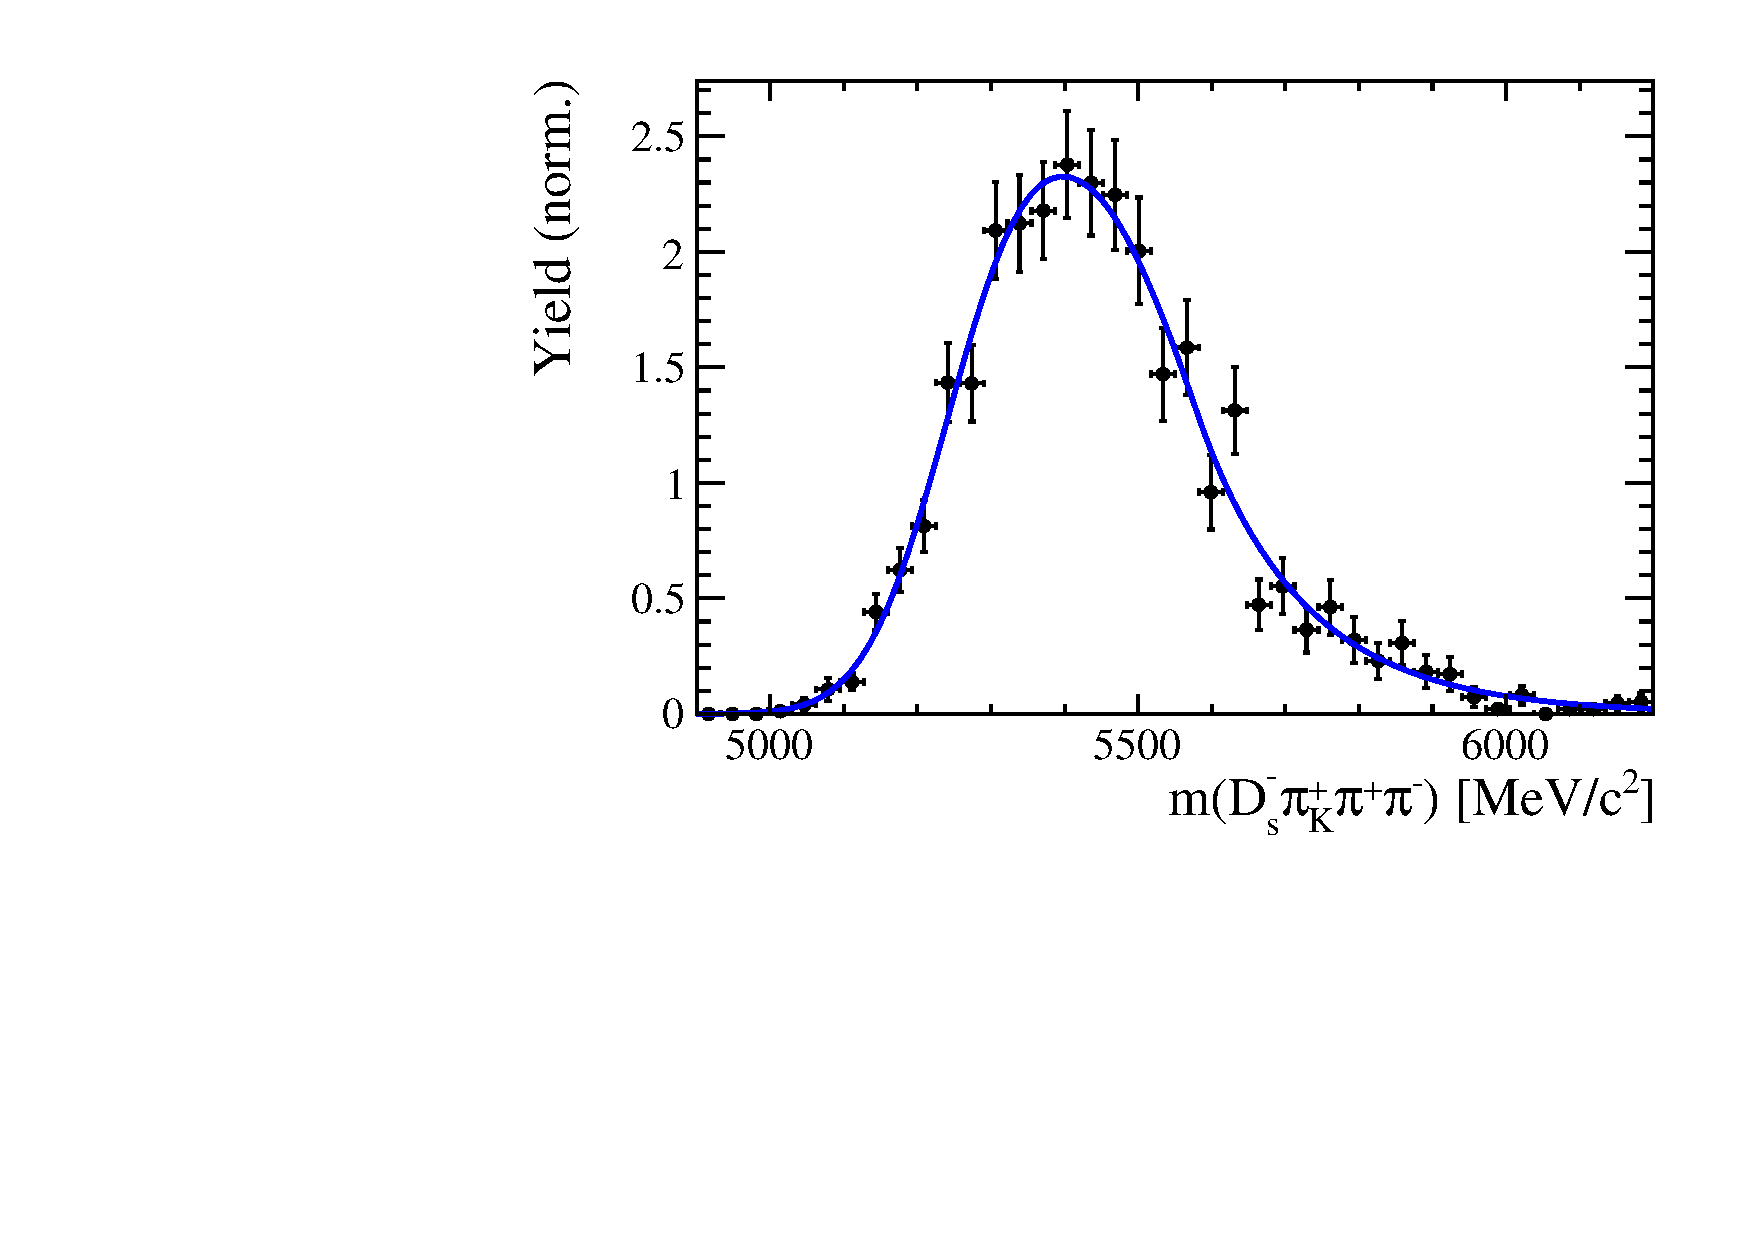
\includegraphics[height=!,width=0.4\textwidth]{figs/MassFit/BkgShape/Bs2Dsstarpipipi_as_DsKpipi_Run1.pdf}
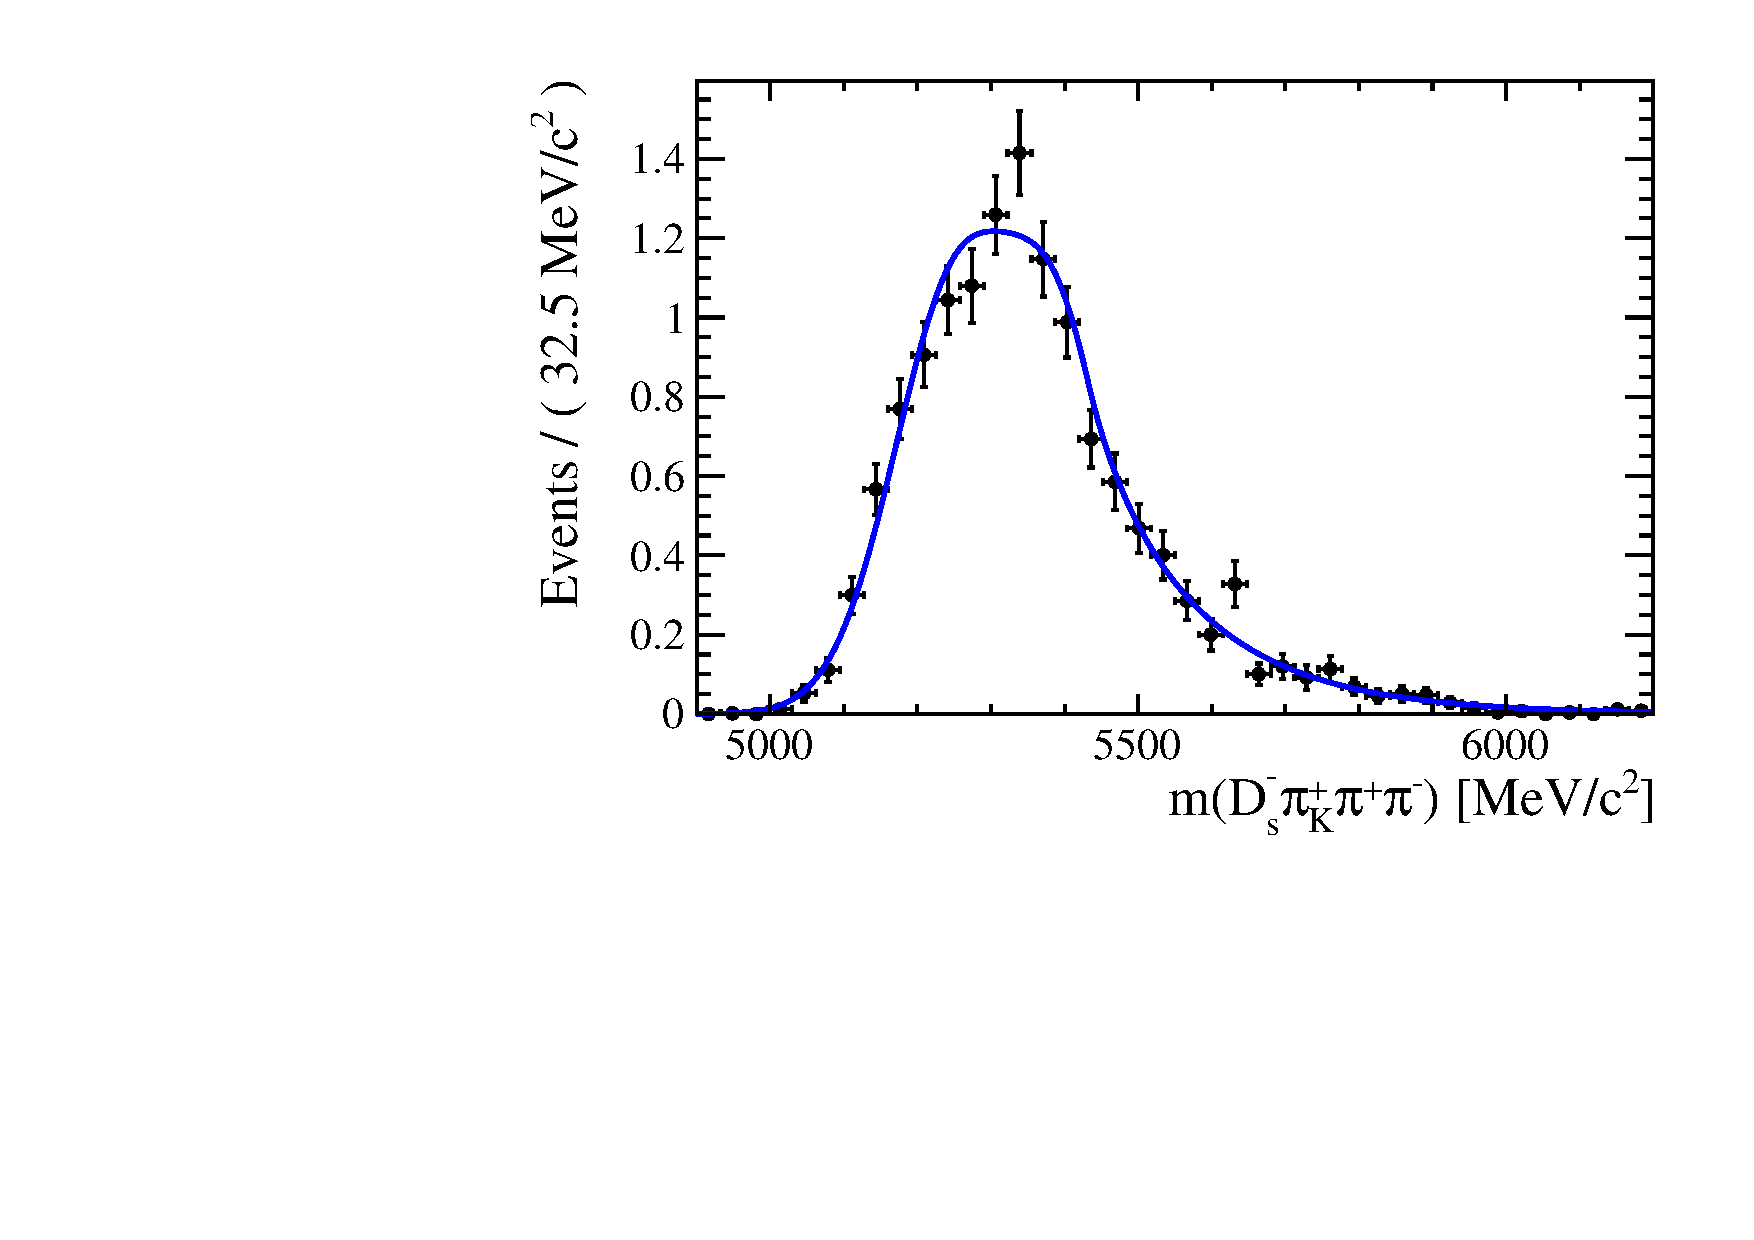
\includegraphics[height=!,width=0.4 \textwidth]{figs/MassFit/BkgShape/Bs2Dsstarpipipi_as_DsKpipi_Run2.pdf}
\caption{
Top: Invariant mass distribution of simulated $\Bs\to D_s^{*}\pion\pion\pion$ events, where the $\gamma$/$\piz$ is excluded from the reconstruction. 
Middle: Invariant mass distribution of  simulated $\Bs\to\Ds\pion\pion\pion$ events for Run-I (left) and Run-II (right), where one of the pions is reconstructed as a kaon taking the misidentification probability into account. 
Bottom: Invariant mass distribution for for simulated $\Bs\to D_s^{*}\pion\pion\pion$ events for Run-I (left) and Run-II (right), where the $\gamma$/$\piz$ from the $D_s^{*}$ is excluded from reconstruction
and one of the pions is reconstructed as a kaon taking the misidentification probability into account. 
The fitted PDFs are shown in blue.}
\label{fig:bgkShapes}
\end{figure}
 
\clearpage
\subsection{Results}
\label{subsec:Results}

Figure \ref{fig:massFit} shows the invariant mass distribution for $\Bs\to\Ds\pion\pion\pion$ and  $\Bs\to\Ds\kaon\pion\pion$ candidates passing all selection criteria.
The projections for all categories of the simultaneous fit are shown in Appendix \ref{sec:DetailedMassfits}. % together with the results for all fitted parameters.
The integrated signal and background yields are listed in Tables \ref{tab:massFitNorm} and \ref{tab:massFitSig}.

\begin{figure}[h]
\centering
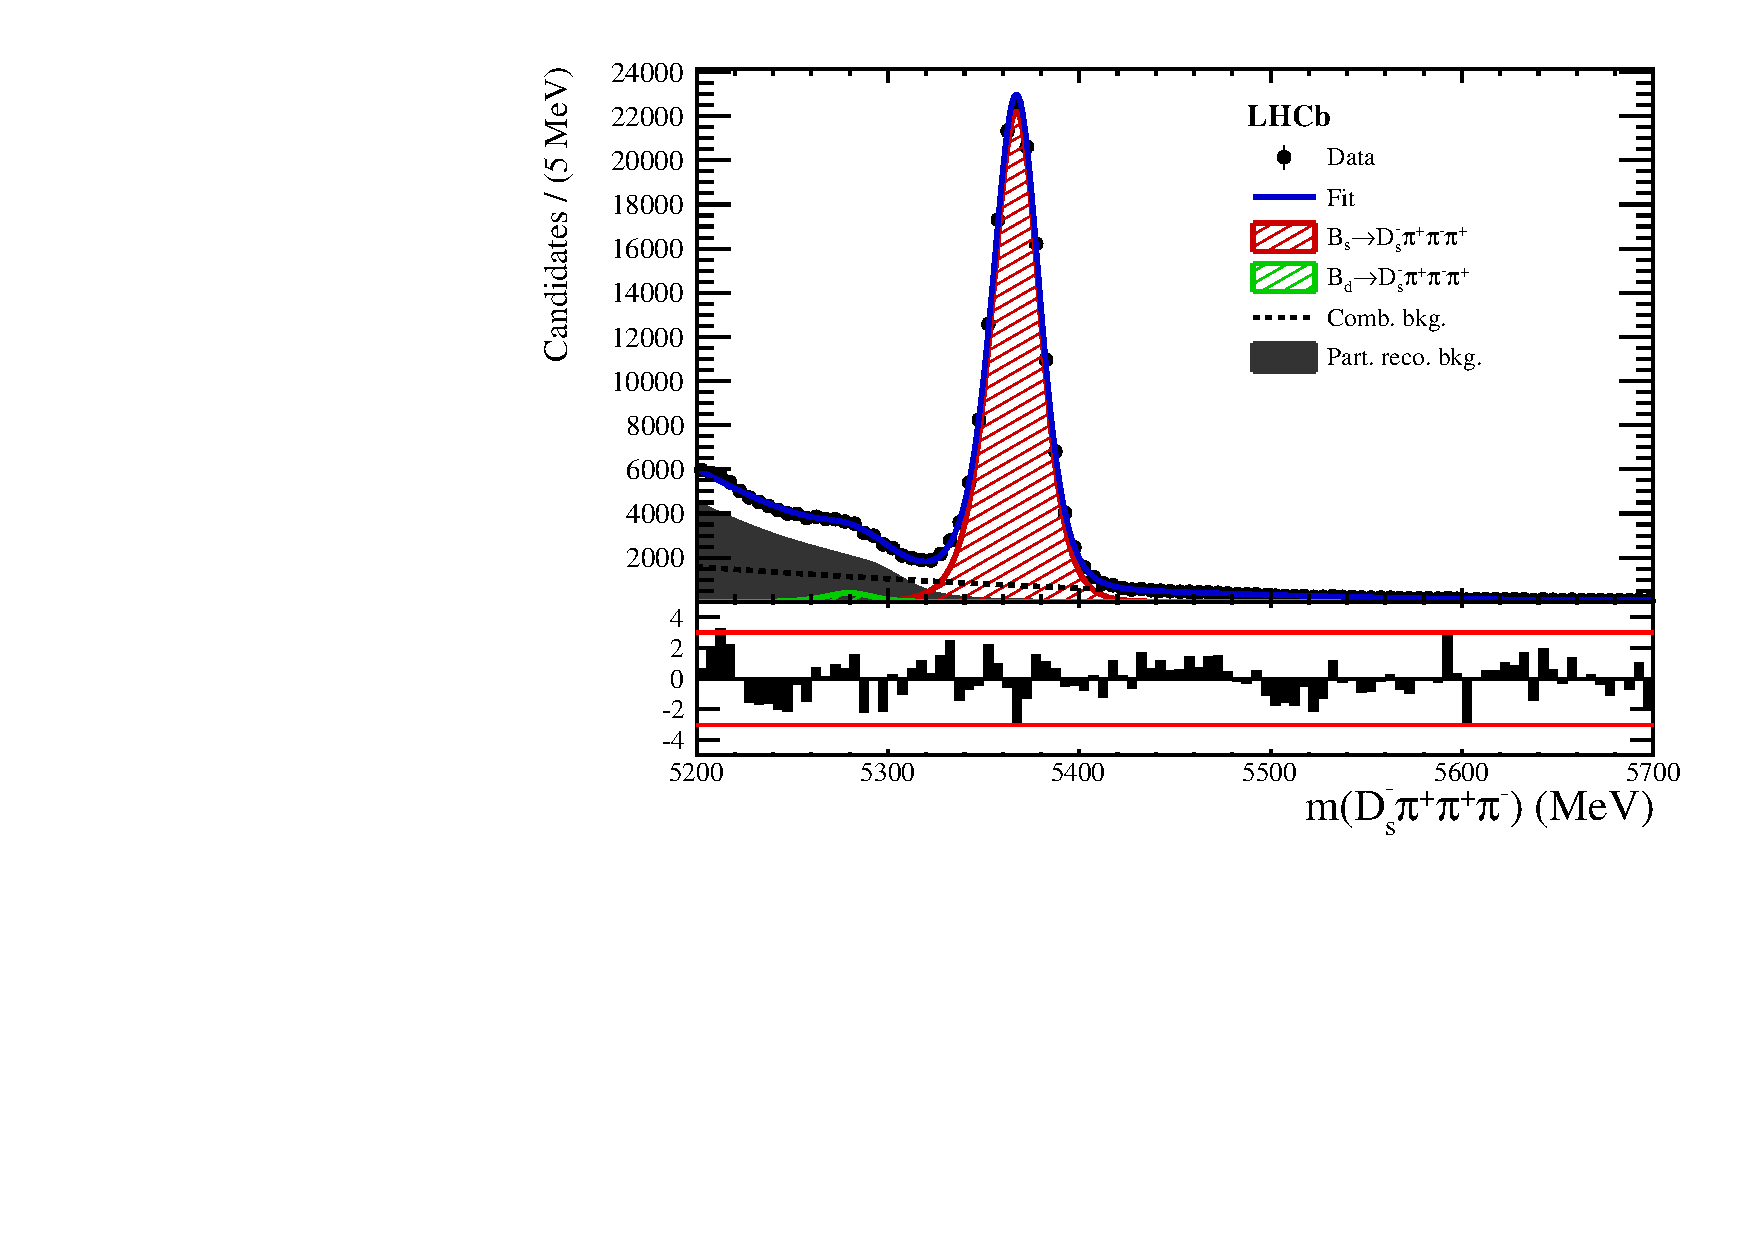
\includegraphics[height=!,width=0.49\textwidth]{figs/MassFit/norm_pull.pdf}
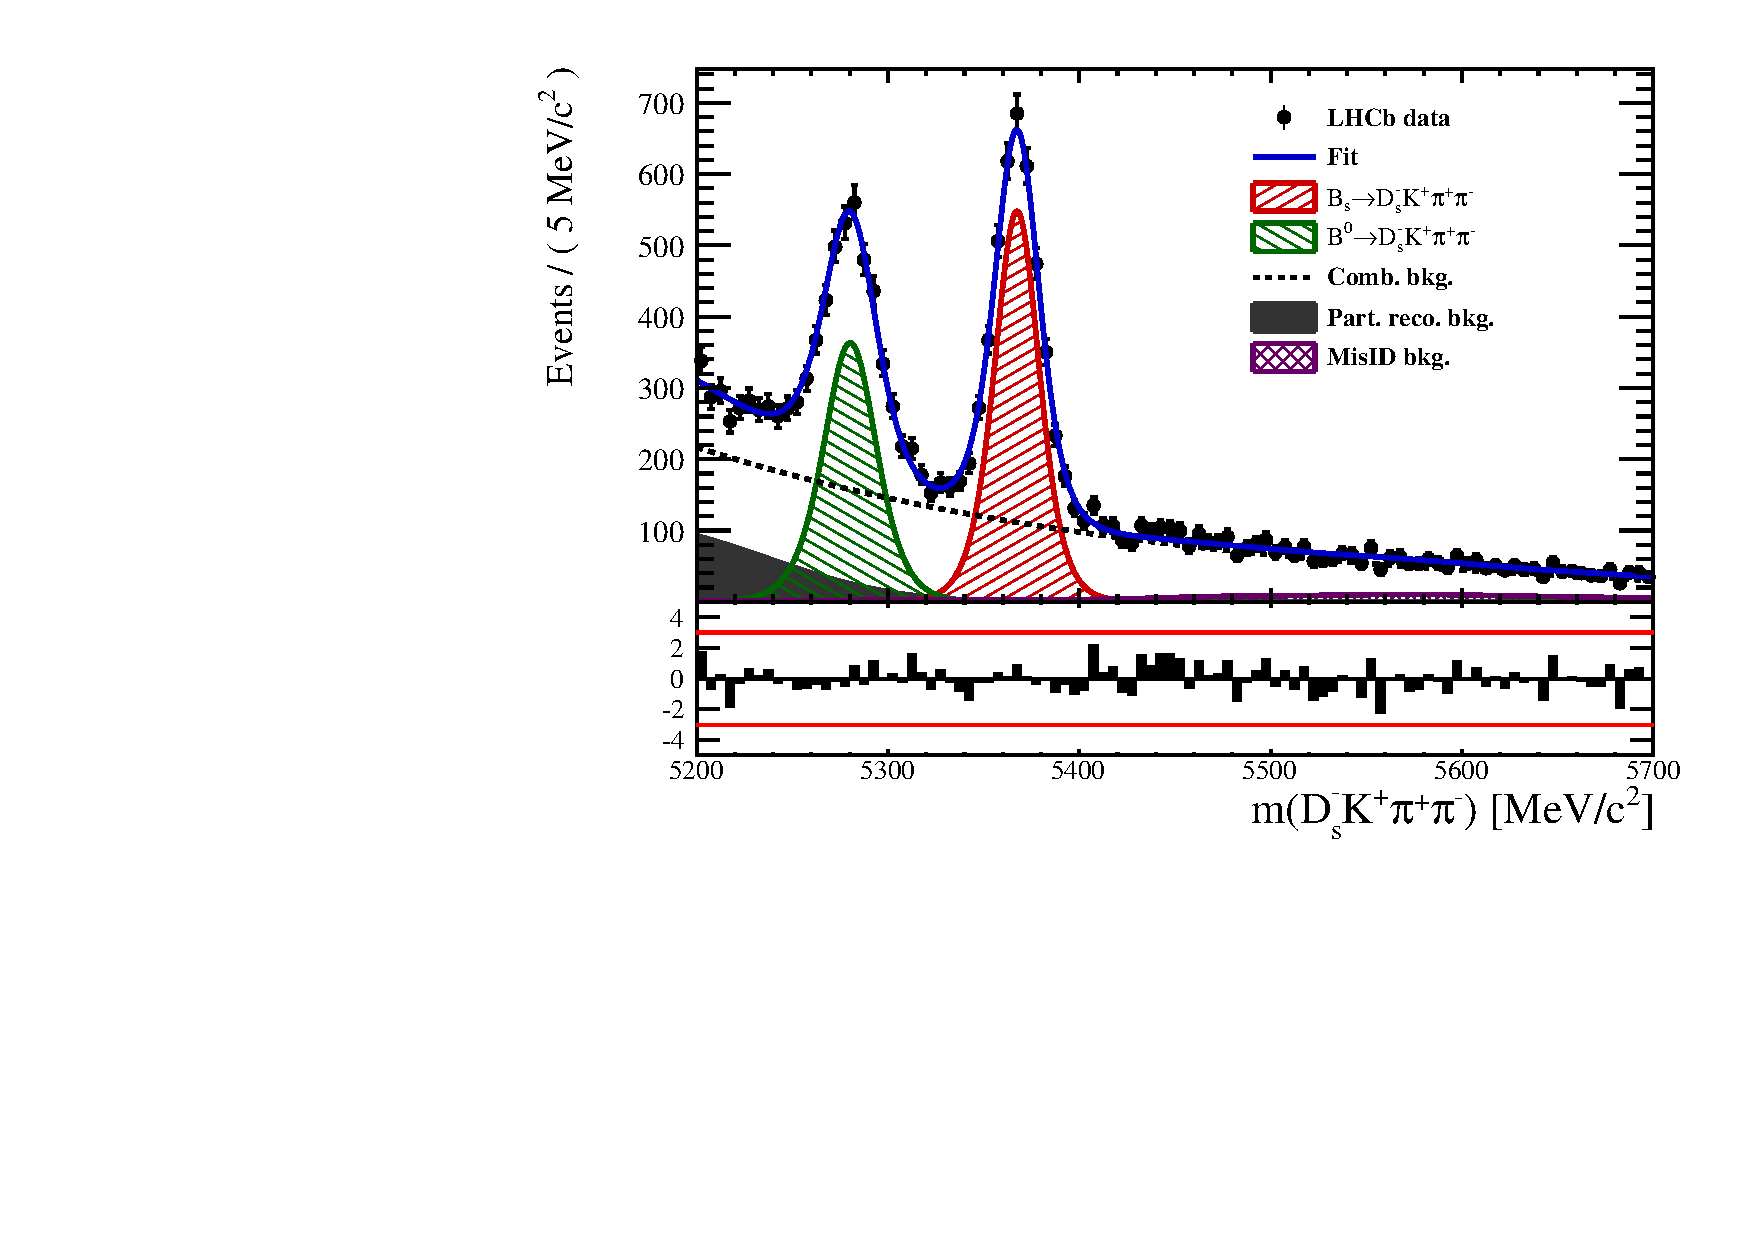
\includegraphics[height=!,width=0.49\textwidth]{figs/MassFit/signal_pull.pdf}
\caption{Invariant mass distribution of $\Bs\to\Ds\pion\pion\pion$ (left) and  $\Bs\to\Ds\kaon\pion\pion$ (right) candidates integrated over all categories.}
\label{fig:massFit}
\end{figure}


\begin{table}[h]
\centering
\caption{Total signal and background yields for the $B_s \to D_s \pi \pi \pi$ sample (left) and
signal yield for the different $D_s$ final states contributing to the $B_s \to D_s \pi \pi \pi$ sample (right).}
 \begin{tabular}{l r }
\hline\hline
Component & Yield\ \\
\hline
$B_s \to D_s \pi \pi \pi$ & 77225 $\pm$ 304 \\
$B^{0} \to D_s \pi \pi \pi$ & 1263 $\pm$ 454 \\
Partially reconstructed bkg. & 31805 $\pm$ 351 \\
Combinatorial bkg. & 32821 $\pm$ 393 \\
\hline\hline
\end{tabular}
\label{table:normYields}
 \hfill
 \begin{tabular}{l r }
\hline\hline
$D_s$ final state  & Signal yield\ \\
\hline
$D_{s}^{-} \to \phi^{0}(1020)\pi^{-}$ & 34563 $\pm$ 197 \\
$D_{s}^{-}\to K^{*0}(892)K^{-}$ & 28472 $\pm$ 189 \\
$D_{s}^{-}\to (K^{-}h^{+}\pi^{-})$ & 21047 $\pm$ 160 \\
$D_{s}^{-}\to \pi^{+}\pi^{-}\pi^{-}$ & 17208 $\pm$ 145 \\
\hline\hline
\end{tabular}
\label{table:normYieldsDs}

\label{tab:massFitNorm}
\end{table}
\begin{table}[h]
\centering
\caption{Total signal and background yields for the $B_s \to D_s K \pi \pi$ sample (left) and
signal yield for the different $D_s$ final states contributing to the $B_s \to D_s  K \pi \pi$ sample (right).}
 \begin{tabular}{l r }
\hline\hline
Component & Yield\ \\
\hline
$B_s \to D_s K \pi \pi$ & 5376 $\pm$ 88 \\
$B^{0} \to D_s K \pi \pi$ & 4384 $\pm$ 101 \\
Partially reconstructed bkg. & 1796 $\pm$ 96 \\
Misidentified bkg. & 808 $\pm$ 0 \\
Combinatorial bkg. & 9376 $\pm$ 177 \\
\hline\hline
\end{tabular}
\label{table:signalYields}
 \hfill
 \begin{tabular}{l r }
\hline\hline
$D_s$ final state  & Signal yield\ \\
\hline
$D_{s}^{-} \to \phi^{0}(1020)\pi^{-}$ & 1728 $\pm$ 49 \\
$D_{s}^{-}\to K^{*0}(892)K^{-}$ & 1575 $\pm$ 47 \\
$D_{s}^{-}\to (K^{-}h^{+}\pi^{-})$ & 1166 $\pm$ 41 \\
$D_{s}^{-}\to \pi^{+}\pi^{-}\pi^{-}$ & 823 $\pm$ 37 \\
\hline\hline
\end{tabular}
\label{table:signalYieldsDs}

\label{tab:massFitSig}
\end{table}


